\newcommand{\implementaras}{Implementatation}

\section*{\implementaras}
\begin{frame}{\modelreality}
Any ideas?
\end{frame}

\def\freqlist{1,2,3,4,5,6,7,8,9}

\foreach \freq in \freqlist 
{
\begin{frame}{\implementaras} 
\begin{figure}
\includegraphics[width=\columnwidth]{input/rasmus/three\freq.pdf}
\end{figure}
\end{frame}
} 

\begin{frame}{\implementaras} 
\begin{figure}
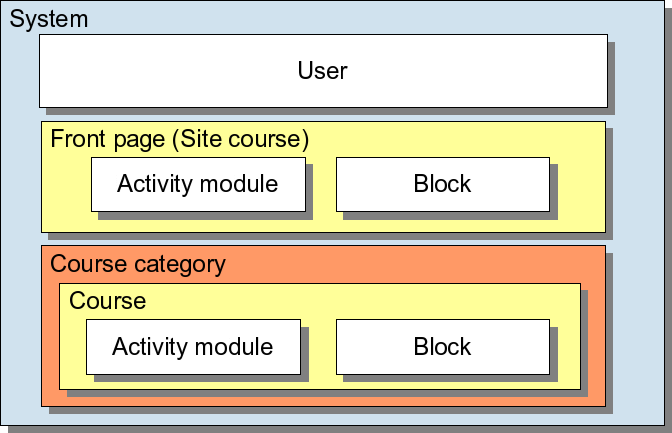
\includegraphics[width=\columnwidth]{input/rasmus/Moodle-contexts.png}
\end{figure}
\end{frame}

\begin{frame}{\implementaras} 
\begin{figure}
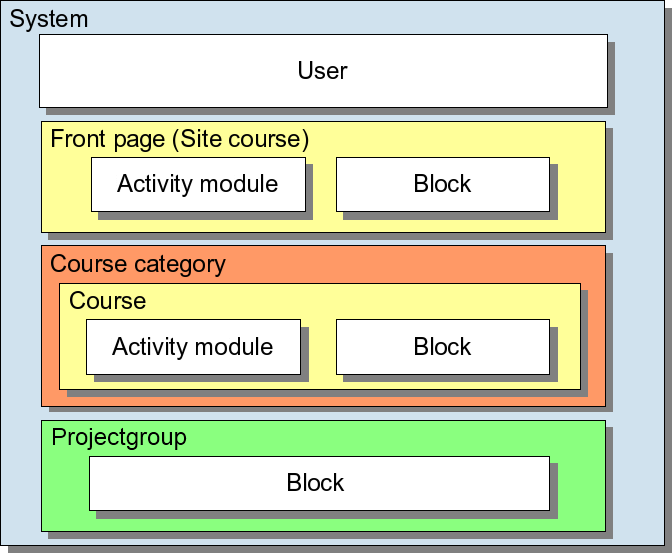
\includegraphics[width=\columnwidth]{input/rasmus/Moodle-contexts-mymoodle.png}
\end{figure}
\end{frame}
